\documentclass[10pt, conference, compsoc]{IEEEtran}
\usepackage{graphicx} % Required for inserting images
\usepackage{authblk}
\usepackage{geometry}
\usepackage{amsmath}

\usepackage{titling}
\newcommand{\subtitle}[1]{%
  \posttitle{%
    \par\end{center}
    \begin{center}\large#1\end{center}
    \vskip0.5em}%
}


\usepackage{parskip}

\def\url#1{\expandafter\string\csname #1\endcsname}

\usepackage{graphicx} %package to manage images
\graphicspath{ {images/} }
\usepackage{caption}

\usepackage[backend=biber]{biblatex}
\addbibresource{sources.bib}
\geometry{margin=1in}

\renewcommand\IEEEkeywordsname{Keywords}

\title{Demand Forecasting by use of\\Long-Short Term Memory (LSTM) Architecture}

\author{Richard Hoehn%
	\thanks{Email: \texttt{rhoehn@mtmail.mtsu.edu}; corresponding author}}
\affil{Middle Tennessee State University\\ \small CSCI 7850\\ \small Prof. Dr. Joshua L. Phillips}

\date{\vspace{1em}\today}

\begin{document}

\maketitle
\thispagestyle{plain}
\pagestyle{plain}

\begin{abstract}
This paper examines the use of Long-Short Term Memory (LSTM), a deep learning recurrent neural network architecture, to predict real-world sales demand. Analyzing five years of daily sales data from ten stores, we prepared the dataset into a univariate temporal single-day format and normalized it using MinMax-Scalers for LSTM training. To mitigate real-world noise, a 7-day rolling average was applied to the daily sales.

Predictions were based on the LSTM model which is frequently used to analyze and predict time-series (temporal) regression problems. The trained LSTM model deployed worked well using a 90-day sequence(s) for training and validation. Since this problem is of a regression type the loss is calculated by use of the Mean-Squared Error (MSE) function with up to 150 epochs during training.

The results, presented in this paper through various plots, demonstrate that the LSTM's predictions closely match actual sales trends, indicating its effectiveness in learning demand patterns and forecasting future sales with a degree of accuracy. Since the predicted values follow the true values, one can infer that the model has good and reliable performance.

The paper concludes with the hypothesis that focusing on individual store data might enhance the model's ability to predict store-specific demand, suggesting a direction for further research.
\end{abstract}

\begin{IEEEkeywords}
LSTM, RNN, Demand Forecast, Deep Learning, Temporal Data, Sales Demand
\end{IEEEkeywords}


\section{Introduction}
In this paper we focused the student learning on demand forecasting, which is the process of predicting future customer demand for products or services using a variety of historical data-points based on a temporal data\footnote{In this project the temporal was daily sales} lineage.

By employing deep learning recurrent neural networks (RNNs) in specific the Long-Short Term Memory (LSTM) architecture the research goal was to provide a model to predict sales demand based on historical daily sales data. The LSTM model is particularly good at capturing complex temporal dependencies over long ranges of time and patterns in historical sales data\cite{pharma-sales-forecast-lstm, predicting-sales-lstm, lstm-gru-performance} making it\footnote{The LSTM Architecture} a very good option for demand forecasting tasks.

The motivation for the this paper is two fold:

\textbf{Firstly}, a time-series problem is very interesting since we often question how an individual or business can predict the future based on past data; additionally how the future might change if the input of said data is changed as a type scenario forecasting exercise.

\textbf{Secondly}, a better understanding of RNNs in specific the LSTM architectures will enhance the student's understanding of this deep learning field and prepare readers for future research in Computation \& Data Sciences with regards to forecasting model designs.

In order to complete this research, data from Kaggle's Demand Forecasting challenge\cite{demand-forecasting-kernels-only} released in 2018 was used. The dataset is comprised of five (5) years of store sales data. Each data point is based on a single day; resulting in the dataset being 912,500 daily sales data points.

The key aims for this project are:
\begin{itemize}
    \item Deploy the dataset in the cloud (AWS) for remote extraction, process, and scrubbing that can then be used for training, validation, testing by the use of LSTM architectures.
    \item Build, Train, and Validate the LSTM model with the pre-processed Kaggle\cite{demand-forecasting-kernels-only} dataset.
    \item \textit{and finally}, using multiple potting techniques provide a visual approach to reviewing the performance of the LSTM model for prediction on the Kaggle\cite{demand-forecasting-kernels-only} dataset.
\end{itemize}

\section{Background}
LSTM models have emerged as a "go-to" tool\cite{pharma-sales-forecast-lstm, predicting-sales-lstm} in the field of demand forecasting. Based on a recurrent neural network's (RNN) architecture, LSTM models are frequently used\cite{pharma-sales-forecast-lstm} to analyze and make predictions based on time-series data, which is a common characteristic in demand forecasting scenarios.

Unlike traditional RNN architectures the LSTM design\cite{understand-lstm} (Fig. \ref{fig:lstm-model}) can regulate the forward and backwards flow of information and more importantly be able to forget non-valuable data-traits. This means that LSTMs can remember pertinent information and utilize patterns from longer\cite{predicting-sales-lstm} historical data, which is an important feature for predicting future sales demand trends that may not be linear in nature\cite{improved-sales-forecasting} or have seasonal traits that need to be captured.

In many of the papers reviewed\cite{pharma-sales-forecast-lstm, predicting-sales-lstm} that used the LSTM architecture on demand forecasts, a tabular / numerical approach to validate the loss and accuracy of their models was used; however this paper uses visual plotting techniques to better gauge the perceived accuracy of these predictive regression problems.


\section{Methods}
In this section the mathematical, theoretical, and practical execution of this paper is introduced and references to the technologies, datasets, and visualization techniques presented.


\subsection{Data Preparations}
The dataset\cite{demand-forecasting-kernels-only} is comprised of five (5) years of store sales data based on 50 different items at 10 different stores. Each data point is a single day's data-point (rows) with this being said the dataset is comprised of 912,500 rows in a \texttt{csv} file.

{\renewcommand{\arraystretch}{2}
\begin{table}[h]
\centering
\begin{tabular}{|rc|rc|}
\multicolumn{4}{c} {\textbf{Dataset Details}} \\  
\hline
  Years       &  5      &  Days            &  1,826 \\ \hline
  Stores      &  10     &  Items per Store &  50    \\ \hline
  Datapoints  & 912,500 & File Type        & csv    \\ \hline
  Min (\$USD) & 11,709  & Max (\$USD)      & 44,936 \\ \hline
  Mean        & 912     & Std.             & 527    \\ \hline
\end{tabular}
\caption{Kaggle Demand Forecast Details}
\label{tab:dataset-details}
\end{table}
}

With the data being a simple tab-based row-column structure we can infer the daily total sales for all stores can be represented as $s$, where each element $s_i$ is the sum of sales across all stores for day $i$.

\begin{equation}
s_i = \sum_{j=1}^{n} a_{ij}
\label{eq:group-sum}
\end{equation}

In this Equation \ref{eq:group-sum} the following is given:
\begin{itemize}
    \item $i$ index for days
    \item $j$ index for stores
    \item $aij$ total sales of store $j$ on day $i$
    \item $si$ total sales across all stores on day $i$
\end{itemize}


\subsection{Smoothing \& Normalization of Dataset}
Based on the description from Kaggle\cite{demand-forecasting-kernels-only} of the data it's evident that it is derived from real-world sources, suggesting it's inherent noise. It is also stated in Kaggle's information that the sales data is in whole US Dollars (\$USD), which means that the values are rather large and are whole (real) numbers in nature. This leads to the need for smoothing and normalization parsing of the data.


\subsubsection{Smoothing}
In order to enhance the demand forecasting capabilities of the model, we used a common smoothing algorithm\cite{improved-sales-forecasting} to help the model learn more easily without the daily noise. A good methodical approach was to use a 7day moving average approach.

\begin{equation}
\text{MA}_i = \frac{1}{7} \sum_{k=i-6}^{i} s_k
\label{eq:moving-average}
\end{equation}

In Equation \ref{eq:moving-average} the details of the moving average are as follows:
\begin{itemize}
    \item $\text{MA}_i$ is the 7-day moving average on day $i$
    \item $sk$ represents the sales on day $k$
    \item The summation $\sum_{k=i-6}^{i} s_k$ calculates the total sales over the 7-day period ending on day $i$ (from day $i-6$ to day $i$)
    \item The factor $\frac{1}{7}$ averages the total sales over these 7 days
\end{itemize}


\subsubsection{Normalization}
Normalization is an important preparation step when preparing sales data for training an LSTM model\cite{improved-sales-forecasting}. This process involves scaling the sales data which is in large whole \$USDs\footnote{See Table \ref{tab:dataset-details}'s Min, Max, \& Std. details} so that it falls within a specific range, typically between $-1 < x < 1$. The purpose of normalization is to ensure that all sales contribute equally to the learning process, preventing some sales data with larger swings (magnitudes) from overpowering\cite{improved-sales-forecasting} the model's learning process.

The process we chose for this project was using the \texttt{MinMaxScaler()}\footnote{Python: \texttt{from sklearn.preprocessing import MinMaxScaler}}, where the minimum value of the data becomes \textsc{-1} and the maximum value becomes \textsc{1}. A formulaic representation of this type scaler can be seen in Equation \ref{eq:min-max-scaler} for details.

\begin{equation}
x_{scaled} = \frac{x-x_{min}}{x_{max}-x_{min}}
\label{eq:min-max-scaler}
\end{equation}

It should be noted that the pre-processing step this research applied is the same as many of the reviewed articles\cite{demand-forecasting-lstm, improved-sales-forecasting} for this paper. Further, many of the reviewed papers\cite{demand-forecasting-lstm} also stated the importance of normalization when training across multiple related time series as the ranges of values of sales demand based projects differ significantly between the temporal series.


\subsection{Sequence Data}
After smoothing and normalization, we divided the data into overlapping 90-day sequences, which is illustrated in Equation \ref{eq:sequence-matrix}. As an example, the first sequence consists of sales data from January 1 to March 31, and then the next from January 2 to April 1, and so on. The target variable for each sequence would be the sales demand following the 90-day period, which in our case is the next day's sales data.

If the target is the sales data for the next day, and you represent the sales data for a single day as $S_t$, then the target for sequence $X_i$ would be $S_{t+1}$, where $t$ is the last day in the 90-day sequence.

\begin{equation}
\mathbf{X}_i = \begin{bmatrix} 
S_{t-89} \\ 
S_{t-88} \\ 
\vdots \\ 
S_t 
\end{bmatrix}
\label{eq:sequence-matrix}
\end{equation}

And for the target variable $y_i$, which is the sales data for the day following the 90-day sequence:

\begin{equation}
\mathbf{y}_i = S_{t+1}
\label{eq:sequence-data}
\end{equation}

These sequence(s) represented in Equation \ref{eq:sequence-data} and their respective target pairs are then split into a 80-20 split for training and validation purposes.


\subsection{LSTM Model \& Training}
The LSTM architecture block diagram shown in Figure \ref{fig:lstm-model} consists of a cell state and three (3) gates: the input gate, which regulates the addition of new information to the cell state; the forget gate, which controls the removal of information irrelevant to the prediction task; and the output gate, which determines what information from the cell state to use in the output.

\begin{figure}[h]
\centering
\captionsetup{justification=centering,margin=1cm}
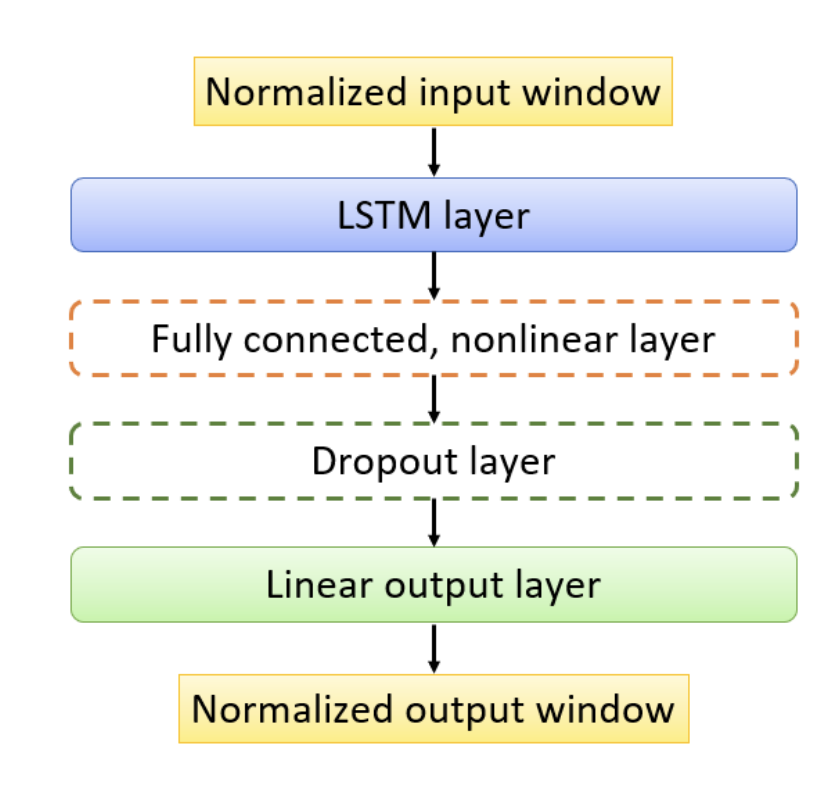
\includegraphics[width=0.3\textwidth]{lstm-network.png}
\caption{LSTM Model used during training}
\label{fig:lstm-model}
\end{figure}

In order for training the Mean Squared Error (MSE) loss function was used. The MSE is often used in regression problems\cite{improved-sales-forecasting} due to it's simplicity, which is the calculated average of the squared differences between the predicted values and the actual values as can be seen in Equation \ref{eq:mse}.

\begin{equation}
\text{MSE} = \frac{1}{n} \sum_{i=1}^{n} (y_i - \hat{y}_i)^2
\label{eq:mse}
\end{equation}

Details of the learning rate we employed for training the LSTM model can me seeing in Figure \ref{fig:mse-loss} and is explained in detail in the following sections (Results \& Discussion) below.


\section{Results}
The subsequent sections are dedicated to presenting both numerical data, used parameters, and visual illustrations that present the work and how it performed in regards to this research.

A substantial amount of the project involved programming, testing, deploying, and training the LSTM model utilizing MTSU\footnote{Middle Tennessee State University}'s High-Performance Computing (HPC) resources.

A general analysis is provided, offering a visual review at the model's performance, including loss over time (Fig. \ref{fig:mse-loss}), as well as other evaluation criteria. In addition to numerical representations, I will include an array of visual aids to convey the general performance of the model, the dynamics of the HPC resource utilization, and the general processes of training and validation. These visuals are designed to enhance the comprehensibility of the data and to bring to light the details of the LSTM's computational work that was performed for this paper.


\subsection{Data Preparation \& Normalization}
As discussed in detail in the methods section of our research, we observed that the Kaggle dataset\cite{demand-forecasting-kernels-only} exhibits significant noise on a daily basis. This noise (see Std. in Table \ref{tab:dataset-details}) can prevent model learning the underlying trends and patterns in the data, making it challenging to extract meaningful sales demand insights.

\begin{figure}[h]
\centering
\captionsetup{justification=centering,margin=1cm}
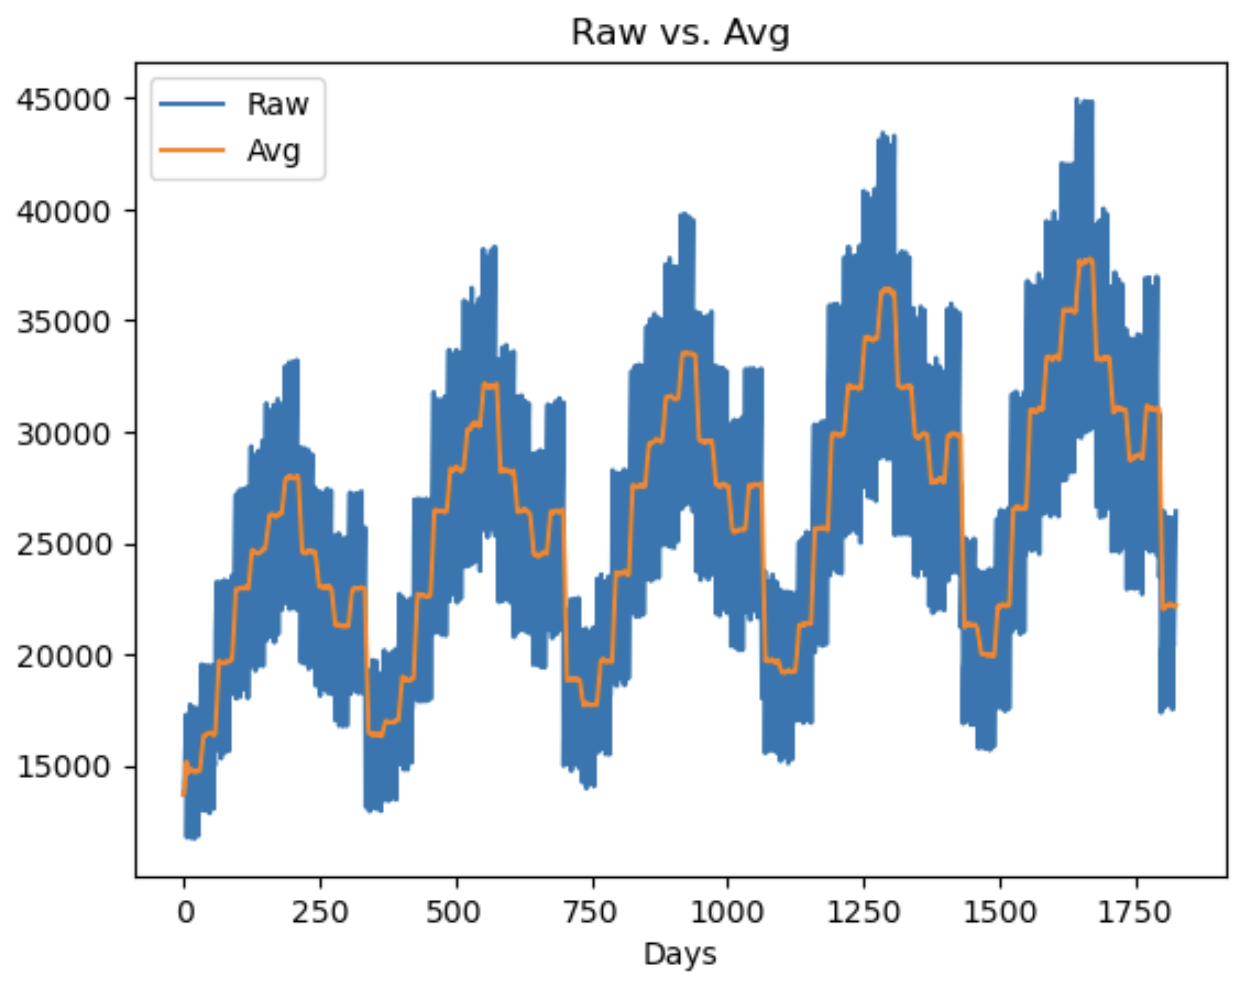
\includegraphics[width=0.45\textwidth]{raw-vs-avg.png}
\caption{Raw (Noise) Data vs. 7-Day Average}
\label{fig:raw-vs-avg}
\end{figure}

To address this issue, we implemented a smoothing technique by calculating a 7-day moving average (see Equation \ref{eq:moving-average} on page \pageref{eq:moving-average}). This approach effectively reduces the daily fluctuations, resulting in a much smoother trend line that more accurately reflects the underlying demand patterns. The impact of this smoothing technique is clearly evident when examining Figure \ref{fig:raw-vs-avg}. The visual shows the blue line representing the raw, un-smoothed data, while the orange line shows the smoothed data using the 7-day average. The comparison between these two lines in the plot highlights the potential effectiveness of the smoothing process, showcasing a more coherent and interpret-able trend in the demand.

\subsection{Model Training \& Hyper-Parameter Tuning}
In Table \ref{tab:hyper-parameters} the used for hyper-parameters in the LSTM model setup are listed. Of note should be that we employed a 4-Layer LTSM model, this is due the us using real-world data, which as described in the Methods section was noisy. Adding more layers\footnote{More than "1" layer is complex} our LSTM model should be more robust to such irregularities, which allows for distinguishing between genuine trends and outliers\cite{pharma-sales-forecast-lstm}. It should be noted that since dropout layer(s) (see Figure \ref{fig:lstm-model} \& Table \ref{tab:hyper-parameters}) are only applied during training, the architecture used in the training phase differs from the one used when performing predictions. The one used during training is schematically illustrated in Figure \ref{fig:lstm-model} on page \pageref{fig:lstm-model}.

{\renewcommand{\arraystretch}{2}
\begin{table}[h]
\centering
\begin{tabular}{|rc|rc|}
\multicolumn{4}{c} {\textbf{LSTM Parameters}} \\  
\hline
  Learning Rate    &  0.001 & Dropout Rate      & 0.1        \\ \hline
  Hidden Layers    &  50    & LSTM Layers       & 4          \\ \hline
  Number of Epochs & 150    & Sequence Size     & 90d        \\ \hline
  Optimizer        & ADAM   & Training (on GPU) & $\sim$6min \\ \hline
  Activation Func. & ReLU   &                   &            \\ \hline 
\end{tabular}
\caption{Hyper-Parameter for LSTM Model}
\label{tab:hyper-parameters}
\end{table}
}

The training time for this compact model was quite brief, averaging only about 6 minutes on the HPC GPUs performing 150 epochs (see Table \ref{tab:hyper-parameters}). It should be noted that the model would based on the MSE-Loss curve perform well at 100 or even less epochs, since both curves in Figure \ref{fig:mse-loss} smooth out at around 80 epochs.

\begin{figure}[h]
\centering
\captionsetup{justification=centering,margin=1cm}
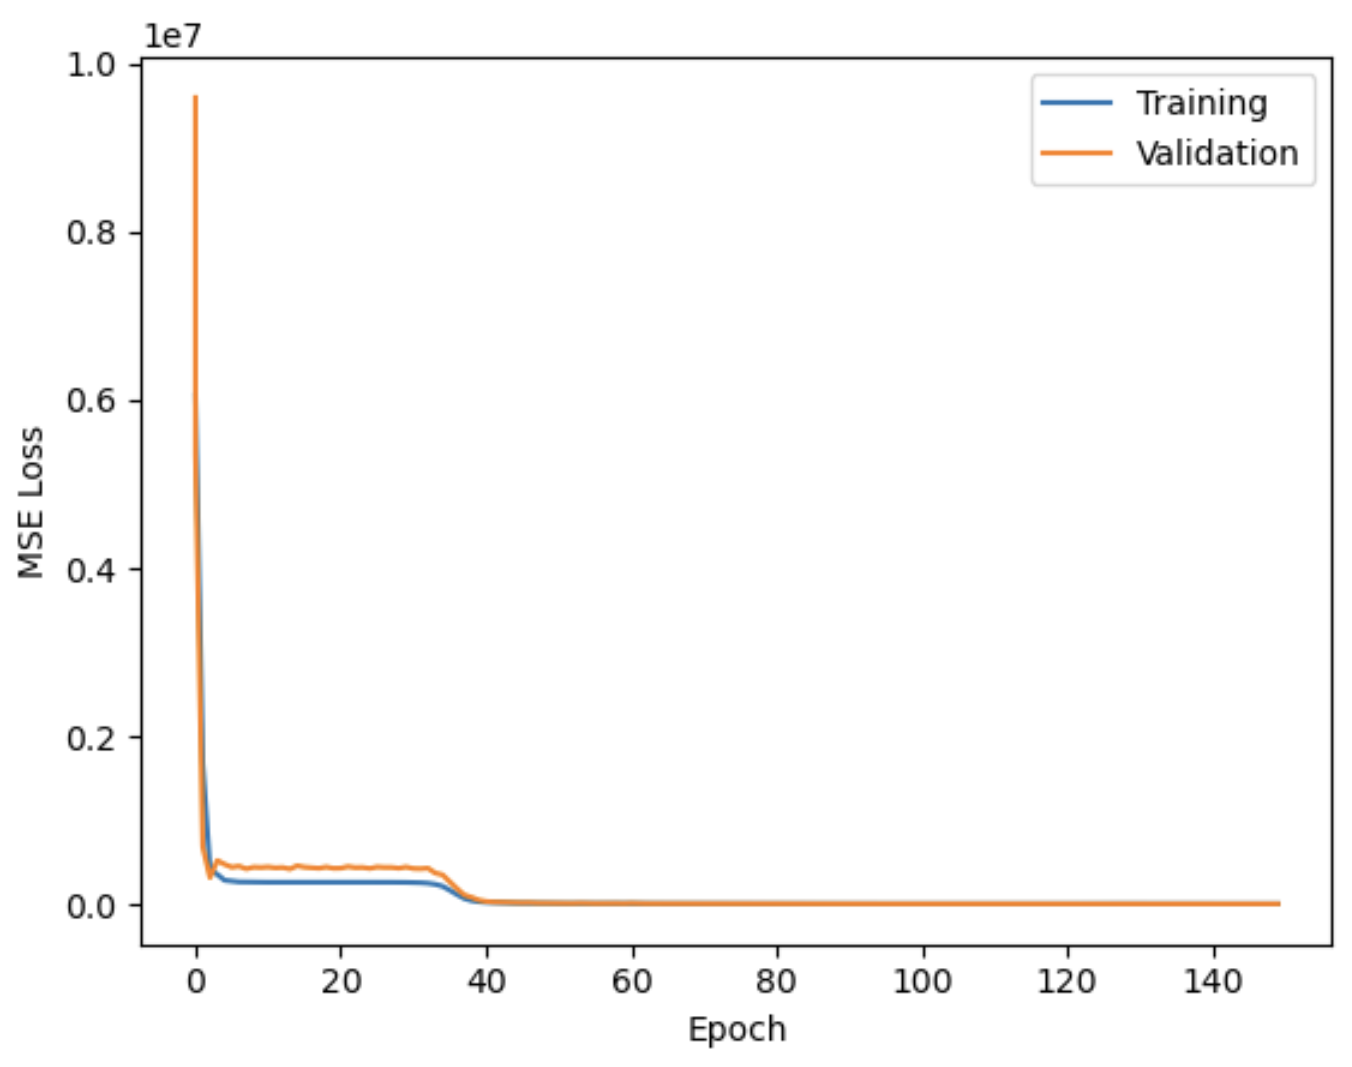
\includegraphics[width=0.45\textwidth]{mse-loss.png}
\caption{MSE Loss Details on Learning}
\label{fig:mse-loss}
\end{figure}

Furthermore, evidence of overfitting was not observed in my analysis (Fig. \ref{fig:mse-loss}), which is indicated by the loss curves for both training and validation. This is most likely a results of us using a dropout rate of $0.1$ (see Table \ref{tab:hyper-parameters}) to prevent overfitting. The curves remained mostly parallel throughout the learning process, suggesting a consistent performance between the training and validation phase. We therefore believe that the parallel trend suggests the model generalized well.


\subsection{Plotting of Actual and Predicted Values}
The training validation of the model are quite promising. Figure \ref{fig:true-vs-predicted} illustrates that it\footnote{The LSTM Model} overall follows the true path during the training and test phases. Overall this trend indicates that both lines follow a similar pattern, with the predicted values closely mirroring the true values. This suggests that the LSTM model has learned the underlying pattern in the training data well and is able to predict the future values with some degree of accuracy.

\begin{figure}[h]
\centering
\captionsetup{justification=centering,margin=1cm}
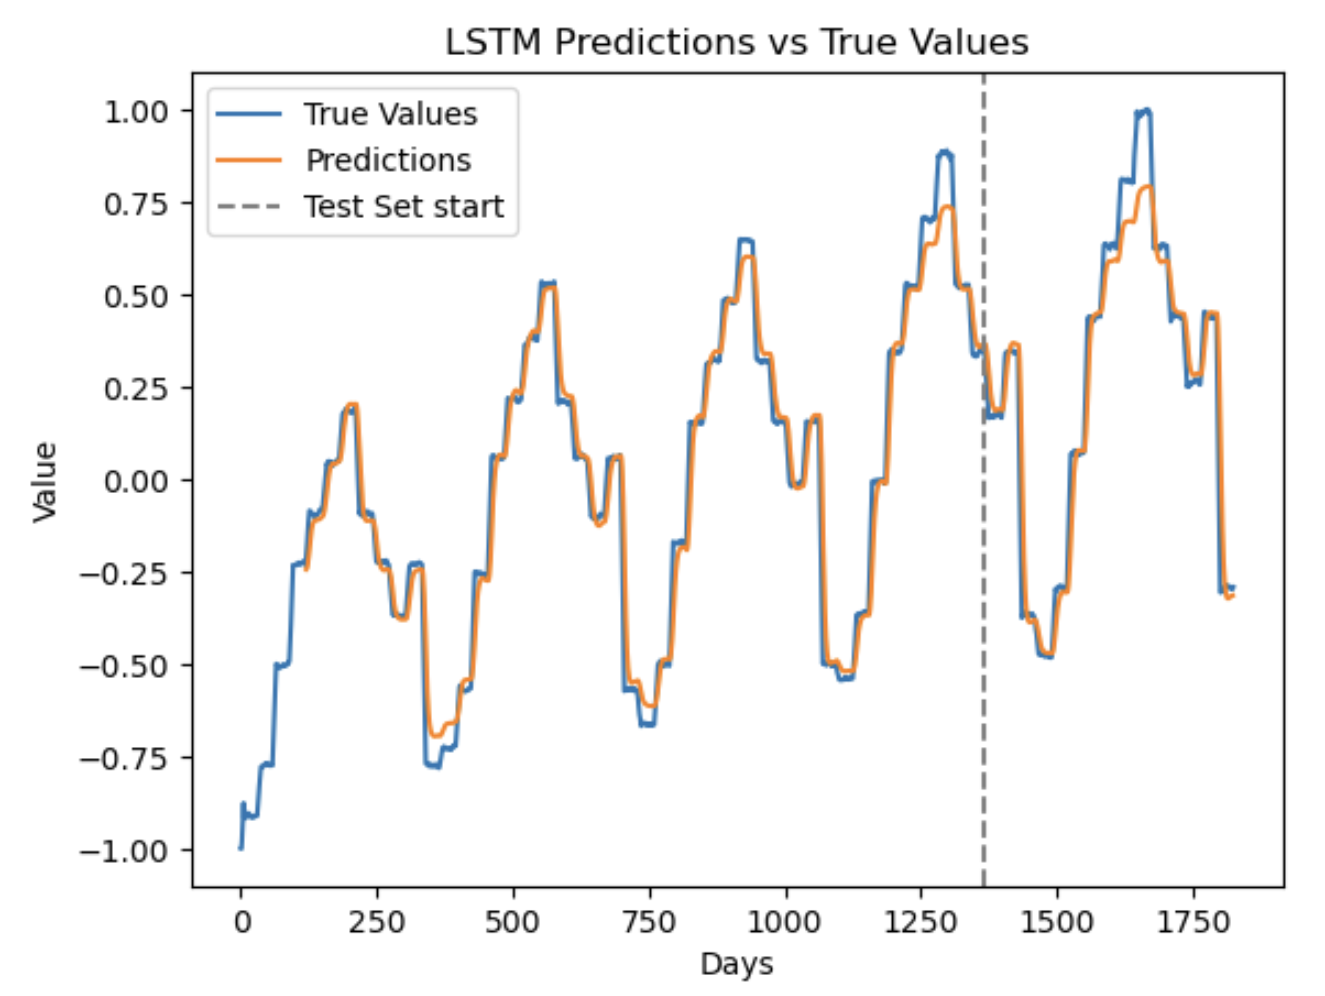
\includegraphics[width=0.45\textwidth]{true-vs-predicted.png}
\caption{True vs. Predicted during training of model}
\label{fig:true-vs-predicted}
\end{figure}



\section{Discussion}
The following section reviews in detail the True vs. Predicted (see Figures \ref{fig:true-vs-predicted} \& \ref{fig:prediction-detail}) results of the LSTM model training. Using separate training and test datasets was critical to ensure that the model learns to generalize from sales demand patterns\footnote{Expl: Seasonality plays a large role in demand forecasts} in the data rather than memorizing it. With this in mind the test data provides an unbiased evaluation of the model's predictive performance on unseen data, reflecting its potential effectiveness in real-world applications. As previously mentioned in Table \ref{tab:dataset-details} on page \pageref{tab:dataset-details} the 80 / 20 split rule was used for training and validation data.

\subsection{Review of Plots}
In Figure \ref{fig:prediction-detail} it is apparent that the LSTM model as able to learn the underlying seasonality of the sales and would therefore be able to predict future demands. However looking closer one can see in Figure \ref{fig:true-vs-predicted} as time moves forward that the difference\footnote{The difference is analogous of the error} between true and predicted values skew higher over time. A more detailed view of this is also displayed in Figure \ref{fig:prediction-detail} on page \pageref{fig:prediction-detail}. 

\begin{figure}[h]
\centering
\captionsetup{justification=centering,margin=1cm}
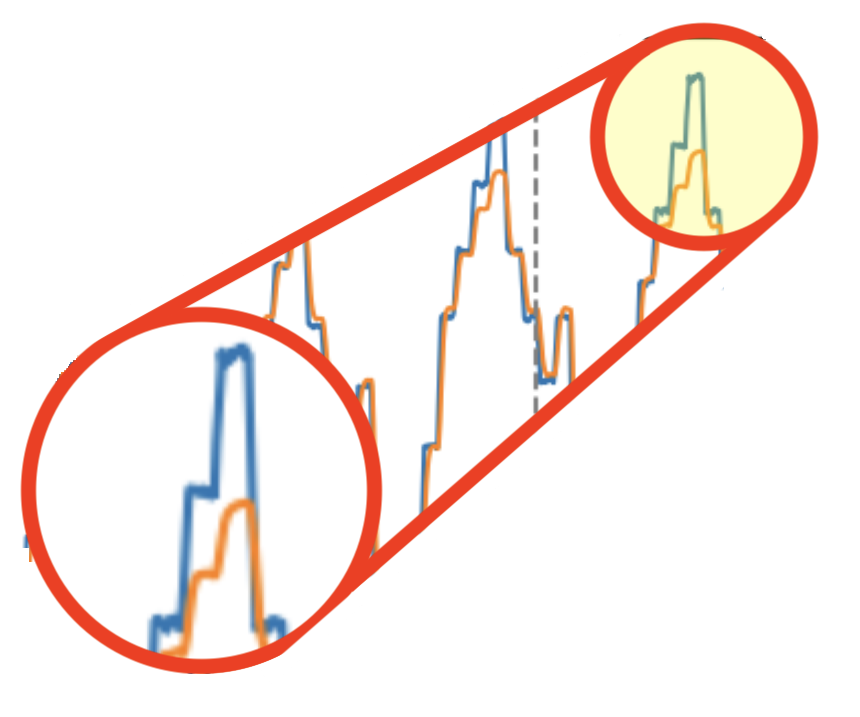
\includegraphics[width=0.45\textwidth]{predicted-detail.png}
\caption{Prediction vs. True detail on peaks}
\label{fig:prediction-detail}
\end{figure}

Overall Trend review indicates that both lines follow a similar pattern, with the predicted values closely mirroring the true values. This suggests that the LSTM model has learned the underlying pattern in the training data well and is able to predict the future values with some degree of accuracy. Since the predicted values closely follow the true values, one could infer that the model has a good performance. 

It should be noted that detail review of the "peak" shows a slight degradation over time from the actual true values. This can be observed in Figure \ref{fig:prediction-detail} in detail as the true (blue) value line peaks higher than the predicted (orange).

\subsection{Future Work}
In order to enhance the demand forecasting capabilities of our models, we anticipate more work to explore the extraction of additional contextual information related to the timestamps, such as seasons, weekdays, holidays, or any other relevant time-based factors. By incorporating these additional features into the dataset, we aim to provide the LSTM model with a richer contextual understanding of the underlying data, which could lead to more accurate predictions.

The strategy here would involve augmenting the dataset with these extracted features and subsequently comparing the performance of the LSTM models with that of the previous non-expanded dataset presented previously. This comparative analysis will shed light on the extent to which the inclusion of more temporal information influences forecasting accuracy.

Lastly, it would certainly be of benefit for the authors to compare the LSTM's predictive output to other similar models such as the Gate Recurrent Unit (GRU) or traditional RNNs models. This would provide additional inference that the LSTM has indeed learned the sales demand from a forecasting and seasonal prediction standpoint.

\clearpage
\section*{Acknowledgments}
We extend our sincere gratitude to the two anonymous reviewers whose insightful comments and constructive critiques improved the quality of this paper. Their expertise and thoughtful feedback have been a great help in refining our research, arguments, and design layout of this paper.


\printbibliography %Prints bibliography
\end{document}
